%%%%%%%%%%%%%%%%%%%%%%%%%%%%%%%%%%%%%%%%%%%%%%%%%%%%%%%%%%%%%%%%%%%%%%%%%%%%%%%%
% Orientation specification
%%%%%%%%%%%%%%%%%%%%%%%%%%%%%%%%%%%%%%%%%%%%%%%%%%%%%%%%%%%%%%%%%%%%%%%%%%%%%%%%

\chapter{Product Specification}\hyperdef{part}{spec}{}\label{ch:spec}

There are many ways to represent the orientation of one three dimensional
object with respect to another. The primary purpose of this model is to
convert between the representation schemes used elsewhere and the schemes
used internally by JEOD.
Figure \ref{fig:representations} portrays the four representation schemes
supported by JEOD. Each of the connections between the representation schemes
in the figure designates a specific method that converts from one scheme
to another. The dotted lines are the responsibility of the \QUATERNION.
The solid lines are the responsibility of this model.

\begin{figure}[hbtp]
\centering
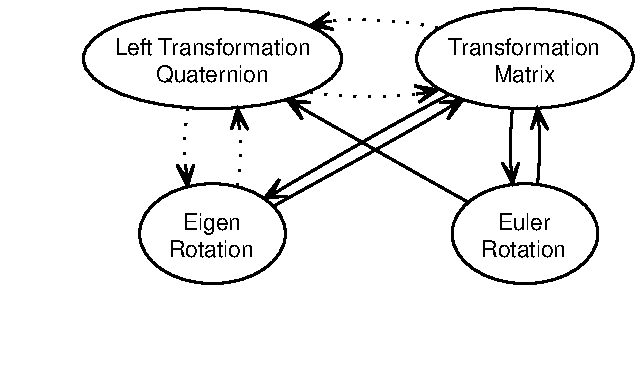
\includegraphics{representations}
\caption{Orientations in JEOD}
\label{fig:representations}
\end{figure}

The representation schemes supported in JEOD are
\begin{itemize}
\item Special orthogonal matrices, or proper transformation matrices.
A proper transformation matrix is an orthogonal matrix whose determinant is one.
The Matrix3x3 class in the \hypermodelref{MATH} provides methods for
manipulating 3x3 matrices and for using them to transform 3-vectors.
Note that JEOD uses transformation matrices rather than rotation matrices.
\item Left transformation unit quaternions.
The unit quaternions are the subject of the \hypermodelref{QUATERNION}.
The Quaternion class defined in that model provides methods that relate to
using unit quaternions to represent rotations and transformations.
Note that JEOD uses left transformation unit quaternions rather than
right quaternions.
\item Eigen axis, or single axis, rotations.
Any sequence of rotations in three dimensional space is equivalent to
a pure rotation about a single axis.
JEOD represents eigen rotations in terms of a rotation angle (a scalar) and a
unit vector that defines the direction of the rotation via the right-hand rule.
\item Euler angles. An Euler rotation sequence is a sequence of three
rotations about a set of principal axes. There are twelve possible conventions
for these rotations. JEOD implements all twelve conventions.
\end{itemize}


\section{Conceptual Design}
The \ModelDesc defines one primary class, the Orientation class.
The model also defines an auxiliary class, the OrientationMessages class, which
member functions of the Orientation class use for error reporting.

\subsection{Static Conversion Methods}
The Orientation class defines static methods which can be used as ordinary
functions to convert between various representations of an orientation.
Each solid line in figure~\ref{fig:representations} represents one of these
static conversion methods provided by the Orientation class.

The graph depicted in the figure is not fully connected. Direct conversions
do exist from all supported representation schemes to both quaternions and
transformation matrices. This is intentional. Other JEOD models use quaternions
and transformation matrices to represent orientations. It is best to have
a direct conversion from all representation schemes to each of the primary
schemes used with JEOD. On the other hand, the eigen rotation and Euler angle
schemes are only partially connected in the figure. This too is intentional.
There is, for example, no driving reason to provide a direction conversion from
eigen rotations to Euler angles. The conversion method would be quite complex
and the conversion can still be made by using a transformation matrix as
an intermediate step.

\subsection{Orientation Objects}
The Orientation class is also instantiable. An Orientation object contains data
members that correspond to each of the four representation schemes supported by
JEOD. The object also contains auxiliary data members that indicate the
representation scheme that was input by the user and that indicate which of the
primary data members have been computed from the user input data.

The class provides several non-static member functions that operate on
Orientation objects. Each method belongs to one the following groups:
\begin{itemize}
\item Constructors.
  The class defines a default constructor and also defines four non-default
  constructors, one per supported representation scheme. One way to initialize
  an Orientation object is to use one of the non-default constructors to
  create the Orientation object.
\item Destructor.
  The Orientation destructor does nothing; orientation objects do not allocate
  resources. The destructor exists so that non-JEOD users can extend the
  class. The Orientation destructor is a virtual destructor.
\item Setters and getters.
  The model provides setters and getters for each of the four supported
  representation schemes, a setter and getter to set/retrieve the Euler
  sequence, and a method to clear (invalidate) the Euler sequence. 
\item Compute methods.
  The member data that describe the supported representation schemes are
  publicly visible. This means outside users can modify the object and
  potentially render it internally inconsistent. The compute methods provide
  the means to make an Orientation object consistent with a specified
  representation scheme.
\item Methods provided by c++.
  Orientation objects do not allocate resources and are not pointers. This
  means that the copy constructor and assignment operator provided by
  default by c++ will work properly.
\item Internal methods.
  The class defines several protected methods that are not available to the
  outside callers. These member functions are protected rather than private,
  so they are accessible to classes that inherit from the Orientation class.
\end{itemize}


\section{Mathematical Formulations}
\label{sec:mathematics}

The mathematics of representing orientations in three space are described in
many references, including Schaub and Junkins\cite{SJ}.
This section focuses on the mathematics that underlies the connections depicted
as solid lines in figure~\ref{fig:representations}. The connections depicted as
dotted lines, the bidirectional conversions between quaternions and matrices and
between quaternions and eigen rotations, are handled by the
\hypermodelref{QUATERNION}. Readers interested in the mathematical formulations
of those conversions should refer to the documentation for that model.


\subsection{Eigen Rotations to Matrices}
Given a pair of reference frames \emph{A} and \emph{B}, with frame \emph{B}
rotated by an angle $\phi$ about an axis $\vhat u$ with respect to
frame \emph{A}, the $i,j$ element of the transformation matrix $\mat T$
from frame \emph{A} to \emph{B} is given by
\begin{equation}
  \label{eqn:eigen_rot_to_mat}
  T_{ij} =
     \cos\phi\,\delta_{ij} +
     (1-\cos\phi)\,\hat u_i \hat u_j +
     \epsilon_{ijk}\sin\phi\,\hat u_k
\end{equation}
where
\begin{itemize}
\item Each of $i$ and $j$ are one of 0, 1, or 2,
\item $k\equiv i+j \bmod 3$,
\item $\delta_{ij}$ is the Kronecker delta,
\begin{flalign*}
  \delta_{ij} &=
  \begin{cases}
     1 & \,\text{if $i = j$} \\
     0 & \,\text{if $i \ne j$}
  \end{cases}
  &&\phantom{0}
\end{flalign*}
\item $\epsilon_{ijk}$ is the Levi-Civita symbol taken with respect to (0,1,2),
\begin{flalign*}
  \epsilon_{ijk} &=
  \begin{cases}
     \phantom{-}1 & \,\text{if $(i,j,k)$ is an even permutation of $(0,1,2)$} \\
     -1 & \,\text{if $(i,j,k)$ is an odd permutation of $(0,1,2)$} \\
     \phantom{-}0 & \,\text{if $i=j$, $i=k$, or $j=k$}
  \end{cases}
  &&\phantom{0}
\end{flalign*}

\end{itemize}

The Levi-Civita symbol vanishes for the diagonal elements while the Kronecker
delta vanishes for the off-diagonal elements. Thus the diagonal elements are
given by
\begin{align}
  \label{eqn:eigen_rot_to_mat_diag}
  T_{ii} &=
     \cos\phi + (1-\cos\phi)\,\hat u_i^2 \\
  \label{eqn:eigen_rot_to_mat_off_diag}
  T_{ij} &=
     (1-\cos\phi)\,\hat u_i \hat u_j \pm
     \sin\phi\,\hat u_k,\,\, j\ne i
\end{align}
Equation~\eqref{eqn:eigen_rot_to_mat_off_diag} is additive
(the $\pm$ becomes +) if $(i,j,k)$ is an even permutation of $(0,1,2)$.
The equation is subtractive for an odd permutation of $(0,1,2)$.

\subsection{Matrices to Eigen Rotations}
The trace of a transformation matrix immediately yields one expression for the
rotation angle.  From equation~\eqref{eqn:eigen_rot_to_mat}, the trace of a
transformation matrix is
\begin{align}
  \label{eqn:eigen_trace}
  \tr \mat T &= 2\cos\phi + 1 \\
  \intertext{Solving for $\cos\phi$,}
  \label{eqn:eigen_trace_phi}
  \cos\phi &= \frac{\tr \mat T -1} 2
\end{align}
The above says nothing about the rotation axis, however.
Each diagonal element does contain information about the corresponding
member of the eigen rotation axis:
\begin{equation}
  \label{eqn:eigen_diag_uhat}
  u_i = \pm\sqrt{\frac{T_{ii} - \cos \phi}{1-\cos\phi}}
\end{equation}
That the sign is unknown (the $\pm$ factor) presents a challenge with
respect to the utility of the above expression.

An alternative expression that contains both the rotation angle and rotation
axis is to look at the symmetric difference of the transformation matrix.
This yields the difference vector $\vect d$,
\begin{align}
  \label{eqn:eigen_sym_diff}
  d_k &\equiv T_{ij}-T_{ji} = 2\sin\phi\,\hat u_k \\
  \intertext{where}
  i &= (k+1)\bmod 3 \nonumber \\
  j &= (i+1)\bmod 3 \nonumber \\
  \intertext{Based on this skew symmetric difference vector,}
  \label{eqn:eigen_sym_diff_phi}
  \sin\phi &= \frac{||\vect d||}2 \\
  \label{eqn:eigen_sym_diff_uhat}
  \vhat u &= \frac {\vect d}{||\vect d||}
\end{align}
Note that equation~\eqref{eqn:eigen_sym_diff_phi} will yield a rotation
angle between 0 and 90 degrees. Special processing will be needed when the
rotation angle is between 90 and 180 degrees.

One final expression is based on the symmetric sum $\mat T + \matT T$.
Given the $i^{th}$ element of the rotation axis unit vector $\hat u_i$, this sum
yields expressions for the other two elements of the rotation axis unit vector:
\begin{align}
  \label{eqn:eigen_sym_sum}
  s_j &\equiv T_{ij}+T_{ji} = 2(1-\cos\phi)\,\hat u_i \hat u_j,\,j\ne i \\
  \intertext{and thus}
  \label{eqn:eigen_sym_sum_uhat}
  \hat u_j &= \frac{s_j}{2(1-\cos\phi)\,\hat u_i}
\end{align}

Summarizing the above, two equations address the rotation angle $\phi$
(equations~\eqref{eqn:eigen_trace_phi} and~\eqref{eqn:eigen_sym_diff_phi})
while three address the rotation axis $\vhat u$
(equations~\eqref{eqn:eigen_diag_uhat}, \eqref{eqn:eigen_sym_diff_uhat},
and~\eqref{eqn:eigen_sym_sum_uhat}). Which is the best to use depends on
the rotation angle. There are four cases to consider.

\paragraph{Null rotations.}
All of the expressions for the rotation axis become indeterminate in the case
of an identity matrix. This case can be easily identified by looking for
$||\vect d||=0$ (equation~\eqref{eqn:eigen_sym_diff}) and $\cos\phi = 1$
(equation~\eqref{eqn:eigen_trace_phi}).
The rotation axis truly is indeterminate in this case. The resolution to this
indeterminacy as implemented in the model code is to arbitrarily say that the
rotation is about the x-hat axis.

\paragraph{Small rotations.}
Small rotations are evidenced by $cos\phi > \sin\phi$, with $\cos\phi$ and
$\sin\phi$ given by equations~\eqref{eqn:eigen_trace_phi}
and~\eqref{eqn:eigen_sym_diff_phi}. This is the region $\phi\in(0,\pi/4)$.
The inverse cosine in this region is less accurate than is the inverse sine,
making equation~\eqref{eqn:eigen_sym_diff_phi} the better choice for determining
the rotation angle. That $\cos\phi$ is somewhat close to one in this interval
means that equations~\eqref{eqn:eigen_diag_uhat}
and~\eqref{eqn:eigen_sym_sum_uhat} are suspect in this region.
Equation~\eqref{eqn:eigen_sym_diff_uhat} is the only viable choice for
determining the rotation axis in this region.

\paragraph{Large rotations.}
Large rotations are evidenced by $-\cos\phi > \sin\phi$. This is the
region $\phi\in(3\pi/4,-\pi]$.  The inverse cosine in this region is again less
accurate than is the inverse sine, once again making
equation~\eqref{eqn:eigen_sym_diff_phi} the better choice
for determining the rotation angle.
In this region it is equation~\eqref{eqn:eigen_sym_diff_uhat} that becomes
suspect for determining the rotation axis.
A combination of equations~\eqref{eqn:eigen_diag_uhat}
and~\eqref{eqn:eigen_sym_sum_uhat} are needed.
Equation~\eqref{eqn:eigen_diag_uhat} will suffer precision loss when the
symmetric sum is close to zero while equation~\eqref{eqn:eigen_sym_sum_uhat}
cannot be used for all three components. The solution is to use
equation~\eqref{eqn:eigen_diag_uhat} for the one component corresponding to
the largest diagonal element of the matrix and to use
equation~\eqref{eqn:eigen_sym_sum_uhat} for the other two components.

Two problems remain in this region. Equation~\eqref{eqn:eigen_diag_uhat} has
a sign uncertainty. Except for rotations very close to 180 degrees,
equation~\eqref{eqn:eigen_diag_uhat} still has enough precision to enable its
use to resolve the sign uncertainty. For rotations of exactly 180 degrees
the choice of axis direction is arbitrary. For rotations very close to 180
degrees getting the sign wrong corresponds to a very small rotation error.
Thus the use of equation~\eqref{eqn:eigen_sym_diff_uhat} to
determine the sign in equation~\eqref{eqn:eigen_diag_uhat} works just fine.
The other problem is that equation~\eqref{eqn:eigen_sym_diff_phi} if
applied directly would yield a small rather than large rotation angle.
This is easily rectified by correcting for the quadrant in which the
angle is known to lie.

\paragraph{Intermediate rotations.}
The remaining cases, $\phi\in[\pi/4,3\pi/4]$, represents the region where
$\sin\phi \ge |\cos\phi|$.
In this region it is equation~\eqref{eqn:eigen_trace_phi} that is more
accurate than equation~\eqref{eqn:eigen_sym_diff_phi}.
Equation~\eqref{eqn:eigen_trace_phi} is used in this region to determine
the rotation angle.  This region is far from the problematic small and large
rotation regions, making the choice of the technique for determining the
rotational axis less pressing. Equation~\eqref{eqn:eigen_sym_diff_uhat} is
used in this to region to determine the rotation because of its simplicity.


\subsection{Euler Angles to Quaternions}
Converting an Euler rotation sequence to a left transformation quaternion is
a very simple process.

An Euler rotation sequence is a sequence of individual rotations, with each
subsequent rotation in the sequence representing a rotation about the
already rotated axes. Since left transformation quaternions chain right to
left, the equation for the left transformation quaternion that results from
an Euler rotation sequence (
$\theta_0$ about $\vhat u_0$,
$\theta_1$ about $\vhat u_1$,
$\theta_2$ about $\vhat u_2$) is
\begin{align}
  \label{eqn:euler_to_quat}
  \quat Q_{\text{seq}} &=
    \quat Q(\theta_2;\vhat u_2)
    \quat Q(\theta_1;\vhat u_1)
    \quat Q(\theta_0;\vhat u_0)
  \intertext{where}
  \label{eqn:euler_to_quat_Q_i}
  \quat Q(\theta_i;\vhat u_i) &=
    \quatsv {\cos\theta_i} {-\sin\theta_i \, \vhat u_i}
\end{align}
Since each element of an Euler sequence is about one of the three principal
axes, forming the unit vectors in equation~\eqref{eqn:euler_to_quat_Q_i} 
is a trivial matter. These are the canonical unit vectors.

\subsection{Euler Angles to Matrices}
The process of converting an Euler rotation sequence to a transformation matrix
is similar to that used for converting an Euler rotation sequence to a left
transformation quaternion. Transformation matrices also chain right to left.
Thus the equation for the transformation matrix that results from an Euler
rotation sequence is
\begin{equation}
  \label{eqn:euler_to_mat}
  \mat T_{\text{seq}} =
    \mat T(\theta_2;\vhat u_2)
    \mat T(\theta_1;\vhat u_1)
    \mat T(\theta_0;\vhat u_0)
\end{equation}
The individual matrices $\mat T_{\theta_i}$ in the above are given by
\begin{align}
  \label{eqn:mat_roll}
  \mat T(\phi; \vhat x) &=
  \begin{bmatrix}
     1 & 0 & 0 \\
     0 & \cos\phi & \sin\phi \\
     0 & -\sin\phi & \cos\phi
  \end{bmatrix} \\
  \label{eqn:mat_pitch}
  \mat T(\theta; \vhat y) &=
  \begin{bmatrix}
     \cos\theta & 0 & -\sin\theta \\
     0 & 1 & 0 \\
     \sin\theta & 0 & \cos\theta
  \end{bmatrix} \\
  \label{eqn:mat_yaw}
  \mat T(\psi; \vhat z) &=
  \begin{bmatrix}
     \cos\psi & \sin\psi & 0 \\
     -\sin\psi & \cos\psi & 0 \\
     0 & 0 & 1
  \end{bmatrix}
\end{align}

\subsection{Matrices to Euler Angles}
A transformation matrix constructed from an XYZ Euler sequence that involves
a rotation of $\phi$ about the X axis, a rotation of $\theta$ about the rotated
Y axis, and a rotation of $\psi$ about the rotated Z axis is of the form
\begin{equation*}
  T_{XYZ} =
  \begin{bmatrix}
     \cos\psi\cos\theta & \cdots & \cdots \\
    -\sin\psi\cos\theta & \cdots & \cdots \\
     \sin\theta  & -\cos\theta\sin\phi & \cos\theta\cos\phi
  \end{bmatrix}
\end{equation*}
Note that $T_{2,0}=\sin\theta$: This element of the matrix depends on
$\theta$ only. The other two elements of the leftmost column are simple terms
that depend on $\theta$ and $\psi$ only, and the other two elements of the
bottommost row are simple terms that depend on $\theta$ and $\phi$ only.
Those five elements are the key to extracting an XYZ Euler sequence from a
typical (non-gimbal locked) transformation matrix.
The same principle applies to all twelve of the Euler sequences:
Five key elements contain all of the information needed to extract the
desired sequence. The location and form of those key elements of course
depends on the sequence.

A problem arises in the above when $\cos\theta$ is zero, or nearly so. This
siutation is called ``gimbal lock''. The four elements used to determine $\phi$
and $\psi$ will be nearly zero in this situation. The elements marked as
$\cdots$ in the above matrix take on a simpler form in this case.
Once again looking at the matrix generated from an
XYZ Euler sequence, when $\theta=\pi/2$ the matrix becomes
\begin{equation*}
  T_{XYZ} =
  \begin{bmatrix}
     0 & \sin(\phi+\psi) & -\cos(\phi+\psi) \\
     0 & \cos(\phi+\psi) & \sin(\phi+\psi) \\
     1 & 0 & 0
  \end{bmatrix}
\end{equation*}
In this case there is no way to determine both $\phi$ and $\psi$; all that can
be determined is their sum. One way to overcome this problem is to arbitrarily
set one of those angles to an arbitrary value such as zero. That is the
approach used in JEOD. This arbitrary setting enables an XYZ Euler
sequence to be extracted from the matrix even in the case of gimbal lock.
The same principle once again applies to all twelve Euler sequences.

In summary, for a transformation matrix corresponding to an XYZ sequence,
\begin{itemize}
\item One element of the matrix, the $[2][0]$ element, specifies $\theta$.
\item The $[1][0]$ and $[0][0]$ elements of the matrix specify $\psi$
   when gimbal lock is not present.
\item The $[1][1]$ and $[2][2]$ elements of the matrix specify $\phi$
   when gimbal lock is not present.
\item The $[1][2]$ and $[1][1]$ elements of the matrix specify $\phi$
   in the case of gimbal lock; $\psi$ is arbitrarily set to zero in this case.
\end{itemize}

One approach to providing the required capability to convert a matrix
to Euler angles would be to write twelve separate conversion methods,
one per rotation sequence. This is not the approach taken in JEOD.
Extending the above analysis to the remaining eleven sequences provides the
essential information needed to extract the Euler angles from a transformation
matrix for any of the twelve Euler sequences. The implementation embeds this
information in a data structure array. Each element of the array
represents one of the twelve sequences and contains
\begin{itemize}
\item The indices of the axes about which the rotations are performed.
  For example, an XYZ sequence entails a rotation about X, then about Y,
  and then about Z. This is a 0-1-2 sequence. A ZXZ seqence is a 2-0-2 sequence.
\item Alternates for the initial and final elements of the sequence.
  For the aerodynamic sequences (XYZ, ZXY, $\cdots$), these alternates
  are just the initial and final elements of the sequence. For the
  astronomical sequences (XYX, XZX, $\cdots$), these alternates are the
  axis that is not involved in the sequence (e.g., Y or 1 for a ZXZ sequence).
\item A boolean that indicates whether the aerodynamic sequence formed by the
  first two elements of the sequence followed by the alternate final element is
  an even (true) or odd (false) permutation of XYZ.
\item A boolean that indicates whether the sequence is an aerodynamics sequence
  (true) or an astronomical sequence (false).
\end{itemize}
The resulting array is
\begin{equation*}
  \begin{array}{c|ccccc}
  \text{Sequence} & \text{Indices} & \text{Alt x} & \text{Alt z} &
    \text{Is even} & \text{Is aero} \\
  \hline
  \text{XYZ} & 0, 1, 2 & 0 & 2 & \text{true}  & \text{true}  \\
  \text{XZY} & 0, 2, 1 & 0 & 1 & \text{false} & \text{true}  \\
  \text{YZX} & 1, 2, 0 & 1 & 0 & \text{true}  & \text{true}  \\
  \text{YXZ} & 1, 0, 2 & 1 & 2 & \text{false} & \text{true}  \\
  \text{ZXY} & 2, 0, 1 & 2 & 1 & \text{true}  & \text{true}  \\
  \text{ZYX} & 2, 1, 0 & 2 & 0 & \text{false} & \text{true}  \\
  \text{XYX} & 0, 1, 0 & 2 & 2 & \text{true}  & \text{false} \\
  \text{XZX} & 0, 2, 0 & 1 & 1 & \text{false} & \text{false} \\
  \text{YZY} & 1, 2, 1 & 0 & 0 & \text{true}  & \text{false} \\
  \text{YXY} & 1, 0, 1 & 2 & 2 & \text{false} & \text{false} \\
  \text{ZXZ} & 2, 0, 2 & 1 & 1 & \text{true}  & \text{false} \\
  \text{ZYZ} & 2, 1, 2 & 0 & 0 & \text{false} & \text{false}
  \end{array}
\end{equation*}

%%%%%%%%%%%%%%%%%%%%%%%%%%%%%%%%%%%%%%%%%%%%%%%%%%%%%%%%%%%%%%%%%%%%%%%%%%%%%%%%
\section{Detailed Design}

The details of the design of the \ModelDesc can be found in the
\hyperref{file:refman.pdf}{}{}
{JEOD Orientation Model Reference Manual} ~\cite{orientation_refman}.


\section{Inventory}
All \ModelDesc files are located in the directory
{\tt \$\{JEOD\_HOME\}/models/utils/orientation}.
Relative to this directory,
\begin{itemize}
\vspace{-0.2\baselineskip}
\item Header and source files are located
in the model {\tt include} and {\tt src} subdirectories.
Table~\ref{tab:source_files} lists the
configuration-managed files in these directories.
\vspace{-0.1\baselineskip}
\item Verification files are located in the model {\tt verif} subdirectory.
See table~\ref{tab:verification_files}
for a listing of the
configuration-managed files in this directory.
\vspace{-0.1\baselineskip}
\item Documentation files are located in the model {\tt docs} subdirectory.
See table~\ref{tab:documentation_files}
for a listing of the
configuration-managed files in this directory.
\end{itemize}

\input{inventory}
